\subsection{Architectures}
\vspace{-10pt}
\begin{figure}[H]
    \centering
    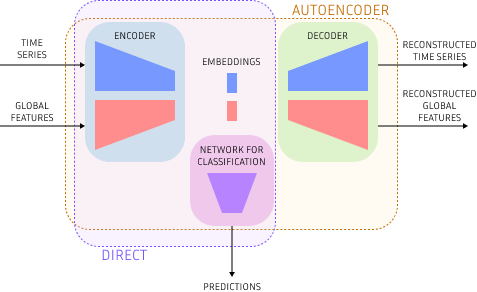
\includegraphics[width=\linewidth]{Deliverables/Report1/img/Architectures.png}
    \vspace{-20pt}
    \label{fig:Architectures}
\end{figure}
% may be removed if too long
%Supported architectures include RNN encoders (multi-layer LSTM/GRU with optional bidirectionality), Conv1D encoders (temporal convolutions with pooling), MultiScaleCNN (parallel convolutional branches at multiple receptive fields), and feedforward classification heads. Additionally if enabled we build a symmetric decoder.
%Supported macroarchitectures are Direct ad Autoencoder.
%The encoder can be recurrent (RNN/LSTM/GRU), Conv1D (temporal convolutions with pooling) or MultiScaleCNN (parallel convolutional branches at multiple receptive fields). A feed forward network performs the classification. If the macroarchitecture is an autoencoder, the decoder is built symmetrically wrt the decoder.
\noindent In our package the supported macro-architectures are Direct (Encoder + FFn) and Autoencoder (AE + FFn).
The encoder may be RNN/LSTM/GRU, Conv1D (temporal convolutions with pooling), or MultiScaleCNN (parallel convolutional branches at multiple receptive fields). If enabled, the decoder mirrors the encoder. Finally, a feed-forward head performs classification.


Starting from the direct architecture (presented in the course) we moved to AEs to further utilize the limited provided data.
%We firstly considered the direct architecture as a baseline presented during the course, and then we added the possibility to use the AE to increase the stability of the embeddings thanks to the reconstruction loss.
In addition, the AE allows us to include the unlabeled test data (almost double the train ones) to help learn meaningful representations while keeping untouched the prediction loss.  
\vspace{-5pt}
\subsection{Pipeline}
\vspace{-5pt}


\noindent Once the dataset is preprocessed, we setup the Optuna study, connecting all the available computational resources (e.g. local, Kaggle and Colab GPUs) to the same experiment in the Database.
The optimization routine executes $n_{\mathrm{trials}}$ and for each, Optuna samples an architecture/hyperparameter configuration among the implemented ones, using a \href{https://optuna.readthedocs.io/en/stable/reference/samplers/generated/optuna.samplers.TPESampler.html}{TPE sampler}. A \href{https://optuna.readthedocs.io/en/stable/reference/generated/optuna.pruners.MedianPruner.html}{Median Pruner} is also used to prune unpromising trials early, saving computational resources.
This allows to reach faster a good configuration compared to the standard grid or Random search.
%The Pipeline module performs architecture selection, $K$-fold cross-validation, checkpointing, distributed training, and submission generation.  
%The system integrates Optuna with TPE sampler and Median Pruner, a DB for persistent experiment tracking, PyTorch Lightning for modular training and logging, and TensorBoard for monitoring.  
%The module supports multiple macro–architectures made of modular micro-architectures.
The sampler also chooses whether to include the global features, to weight the loss with the class weights and to perform windowing.

For each sampled configuration, Stratified K-fold cross-validation is applied with $K=5$. For each fold, the pipeline (using the dataloader class) splits train and validation data, including the test data if the sampled macro-architecture is
an AE and optionally loads the global features.
The architecture is built using the sampled configuration and trained with AdamW to minimize a convex combination of the Reconstruction and the Prediction loss (MSE, cross-entropy). Stochastic Weighted Averaging \href{https://pytorch.org/blog/stochastic-weight-averaging-in-pytorch/}{(SWA)} and Gradient Clipping \href{https://docs.pytorch.org/docs/stable/generated/torch.nn.utils.clip_grad_norm_.html}{(GC)} are added to enache the training stability. We used \href{https://lightning.ai/}{Pytorch Lightning} as a way to simplify model training, checkpointing and logging (using Tensorboard).
After each trial the F1Score is computed averaging the best checkpoints for every fold. 

When we decide to stop the study, the best model is chosen as the one that maximizes that metric, and the selected configuration (model + weights) is used to compute the predictions on the test data to generate the submission CSV.
Optionally, we can retrain the best model and create an ensemble model where each sub-model is the best checkpoint for every fold.

%Given the datasets $X \in \mathbb{R}^{N \times F \times T}$, $G \in \mathbb{R}^{N \times D}$,the pipeline automates the selection of model parameters $\theta$, trained via cross-validation to maximize a validation metric (mean F1-score). The optimization routine executes $n_{\mathrm{trials}}$. For each trial \(j\), Optuna samples a hyperparameter configuration$\theta^{(j)} \sim q(\theta \mid \mathcal{S}),$ where $q$ is the TPE-induced density estimator. The objective function evaluates the metrics across $K$ folds:$\mathcal{L}(\theta^{(j)}) = \frac{1}{K} \sum_{k=1}^K \mathrm{F1}_{\mathrm{val}}^{(k)}(\theta^{(j)}).$

%Each fold involves the creation of training/ validation splits, construction of encoder/ decoder/ head modules according to $\theta^{(j)}$, application of He initialization 
%$W \sim \mathcal{N}\!\left(0, \frac{2}{\mathrm{fan\_in}}\right),$
%, optional wrapping in a windowed model, and PyTorch Lightning training with early stopping and checkpointing. The pipeline generate predictions 
%$
%P \in \mathbb{R}^{N_{\mathrm{test}} \times C},
%$
%%applies aggregation rules, converts class indices to textual labels, and creates the final CSV. 

%Additional utilities include validation of parameter configurations, ensemble model support, feature-selection wrappers, and automatic He initialization.

